\subsection{K nearest neighbors density}
An approach which does not use probability, is k-nearest neighbors (KNN). This method calculates the average distance to the $K$ nearest neighbors and uses the reciprocal value as a density measure.

\begin{equation}\label{eq:KNN}
    \text{density}_{\mathbf{X}_{\setminus i}} (\mathbf{x}, K) = \frac{1}{\frac{1}{K} \sum_{\mathbf{x'}\in N_{\mathbf{X}_{\setminus i}} (\mathbf{x}, K)} d(\mathbf{x}_i, \mathbf{x'})}
\end{equation}

Both the number of nearest neighbors and the distance measure must be specified when applying the method. The distance measure in this case is the euclidean distance, and since we cannot find the optimal amount of nearest neighbors for the data set through e.g. cross validation in this case, we combine the models for all values of $K$ up to $N$, similar to ensemble methods from section 15 in the course notes \cite{coursenotes}. The resulting density score and distribution is seen in figures \ref{fig:KNN_DensityScore} and \ref{fig:KNN_DensityDistribution} similar to what we saw with the KDE method. The interval for the density scores is $[22.3, 261]$
\begin{multicols}{2}
\begin{figure}[H]
    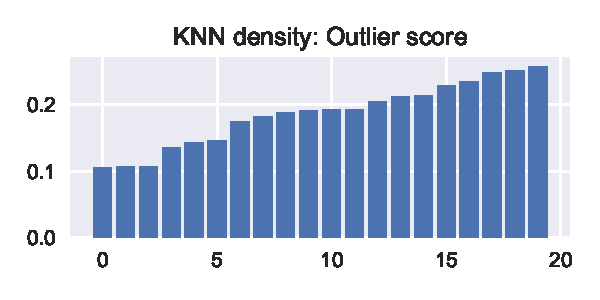
\includegraphics[width=\linewidth]{fig/KNN_densitybarplot_lowest20.pdf}
    \caption{20 lowest density scores using eq. \eqref{eq:KNN}.}
    \label{fig:KNN_DensityScore}
\end{figure}

\begin{figure}[H]
    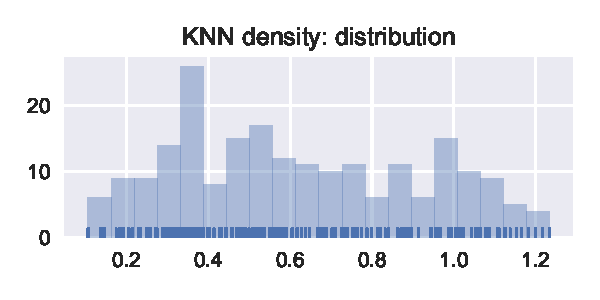
\includegraphics[width=\linewidth]{fig/KNN_densitydistribution.pdf}
    \caption{Density score distribution for the entire data set.}
    \label{fig:KNN_DensityDistribution}
\end{figure}
\end{multicols}

This method does not differentiate between clusters in high or low density areas either. The interval of density scores is not as extreme as with KDE, since the densities are based on the euclidean distance, and is not exponentially dependent. 

